\chapter{Simulation Results}
\newcommand\simResultFigSize{0.7}
\label{chap-five}

We have used Qrsim quadrotor simulator \cite{denardi2013rn} - briefly explained in Section \ref{qrsim_intro} - for evaluating our protocol. The volume of the simulated flying zone is 120 units $ \times \text{120 units} \times \text{120 units, out of which we have used 80 units} \times \text{80 units}\times $ 40 units where drones can be placed. We also have a scaling factor which scales the simulation units i.e. a scaling factor of 5 will make 1 unit in simulation to 5 meters. The drones have a reliable transmission range of $\approx 90 m$ (\fref{fig:packet_loss}) and the wi-fi antenna is omnidirectional. The simulation state changes at a time quantum of 0.2 seconds.

Initially, the drones start in a mesh formation arranged in a 2D grid as shown in \fref{fig:mesh_formation} and gradually they wrap around the plume - which, in our case, for simplicity, has been assumed to be spherical \fref{fig:final_state}. Besides these two formations, we have also evaluated our results for a random distribution of drones in the simulation space \fref{fig:random_formation}.

\begin{figure}[hbtp]
\centering
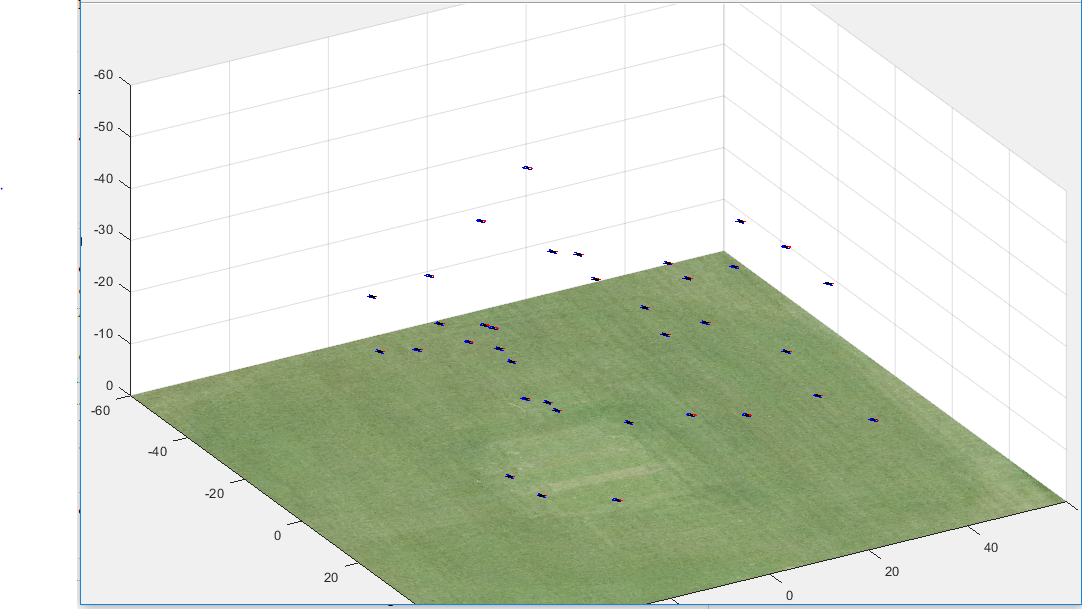
\includegraphics[width=0.5\textwidth]{ncsuthesis-0.6/Chapter-5/figs/random_drone_locations}
\caption{Random distribution of UAVs in the simulation space}
\label{fig:random_formation}
\end{figure}

The messages sent among the drones are assumed to be small and we have not considered transmission errors and congestion separately, rather they are assumed to be represented by the free space path loss model explained in Section \ref{free_space_path_loss} and the parameters which are in Table \ref{tab:fspl_parameters}. 

In the following sections we compare the performance of our routing scheme to flooding. We shall be studying the following performance metrics `Packet delivery ratio', `Average end-to-end delay', `Average number of hops', `Average number of transmissions' \cite{OUBBATI201729}:

We compare these metrics for three arrangements of the UAVs namely, \emph{mesh} - \fref{fig:mesh_formation}, \emph{random} - \fref{fig:random_formation}, \emph{spherical} - \fref{fig:final_state}. The three formations have peculiar properties, for example the spherical formation has the plume acting as a \emph{routing void}, whereas the mesh formation represents a 2D formation and thus we can study the performance of our 3D routing scheme in a 2D setting. Finally, random placement of the drones lets us study the performance in a generic situation. We have presented the results for 1000 packet transfers between two furthest nodes. In appendix we have presented the plots for the mean and standard error for 10 such iterations.

\section{Packet delivery ratio}
\label{pdr}

\begin{figure}[hbtp]
\centering
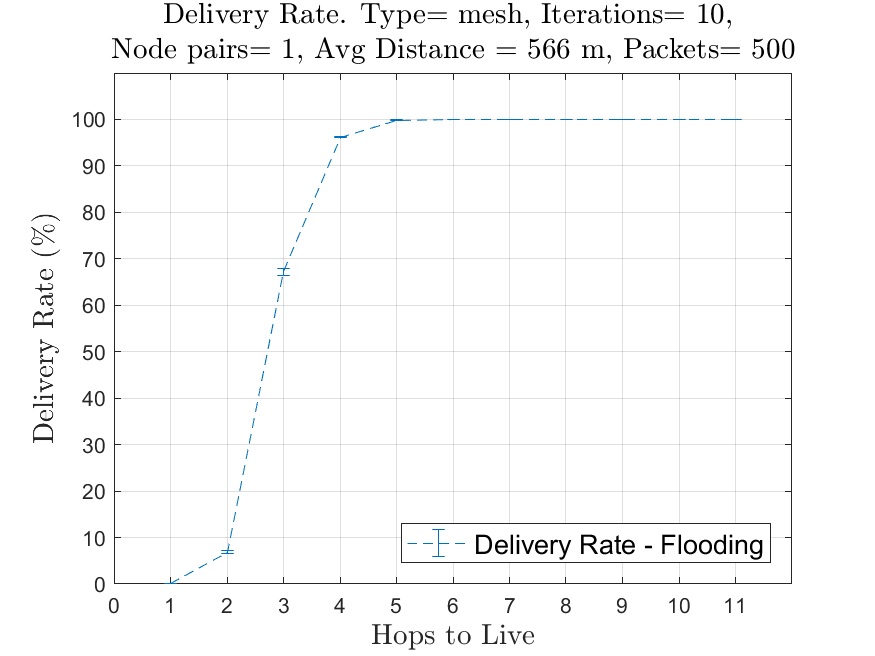
\includegraphics[width=\simResultFigSize \textwidth]{ncsuthesis-0.6/Chapter-5/figs/fl_DR_mesh.png}
\caption{Delivery rate in mesh formation for flooding}
\label{fig:fl_DR_mesh}
\end{figure}

\begin{figure}[hbtp]
\centering
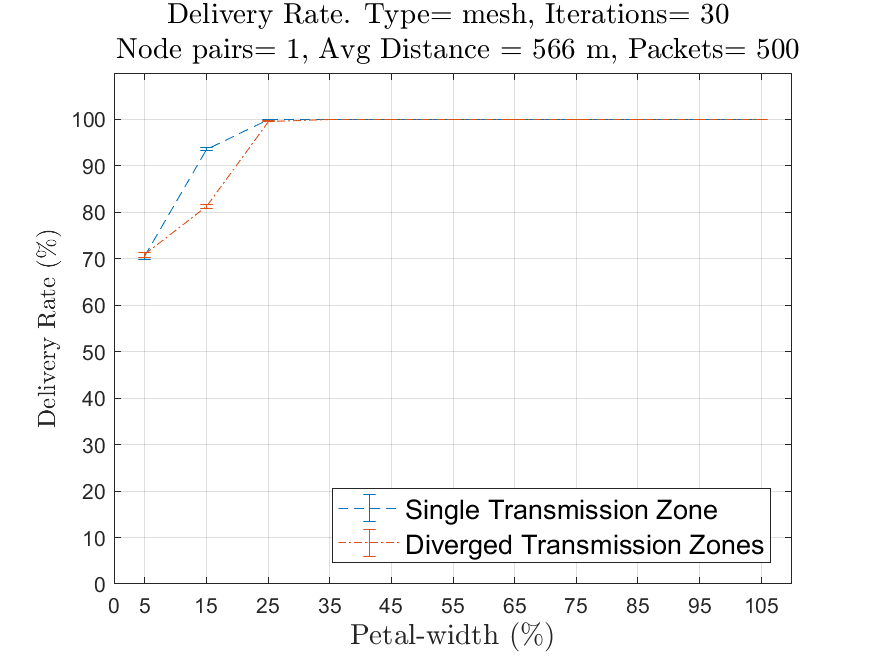
\includegraphics[width=\simResultFigSize \textwidth]{ncsuthesis-0.6/Chapter-5/figs/pe_DR_mesh.png}
\caption{Delivery rate in mesh formation for petal routing}
\label{fig:pe_DR_mesh}
\end{figure}

\begin{figure}[hbtp]
\centering
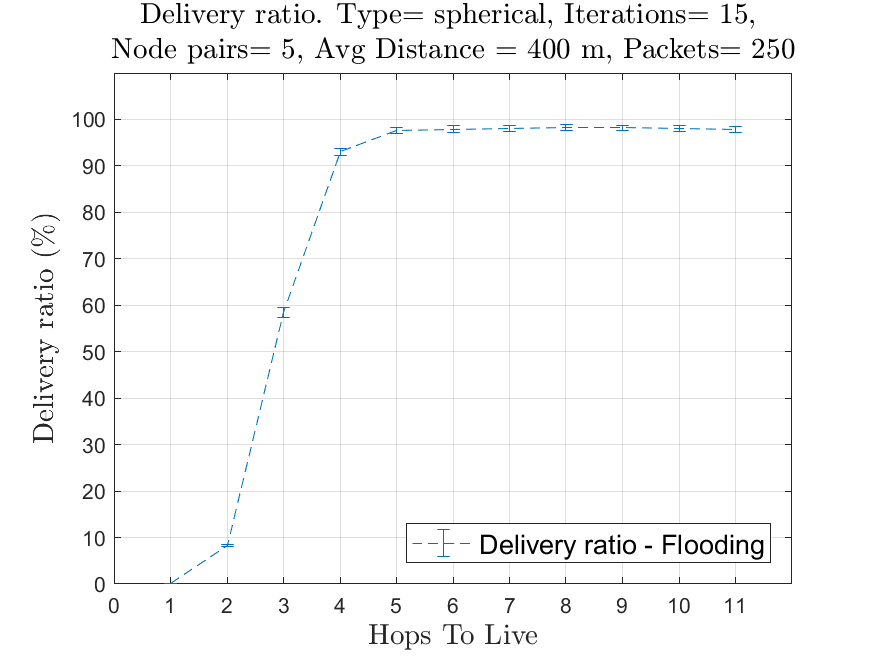
\includegraphics[width=\simResultFigSize \textwidth]{ncsuthesis-0.6/Chapter-5/figs/fl_DR_spherical.png}
\caption{Delivery rate in spherical formation for flooding.}
\label{fig:fl_DR_spherical}
\end{figure}

\begin{figure}[hbtp]
\centering
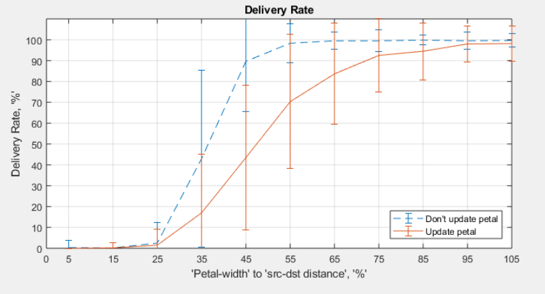
\includegraphics[width=\simResultFigSize \textwidth]{ncsuthesis-0.6/Chapter-5/figs/pe_DR_spherical.png}
\caption{Delivery rate in spherical formation for petal routing.}
\label{fig:pe_DR_spherical}
\end{figure}

\begin{figure}[hbtp]
\centering
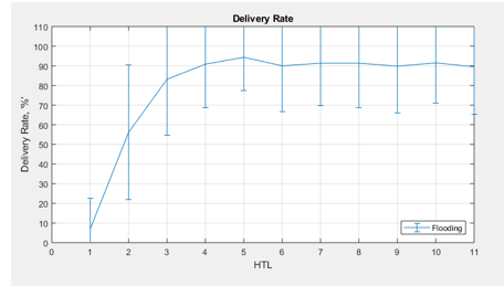
\includegraphics[width=\simResultFigSize \textwidth]{ncsuthesis-0.6/Chapter-5/figs/fl_DR_random.png}
\caption{Delivery rate in random formation for flooding}
\label{fig:fl_DR_random}
\end{figure}

\begin{figure}[hbtp]
\centering
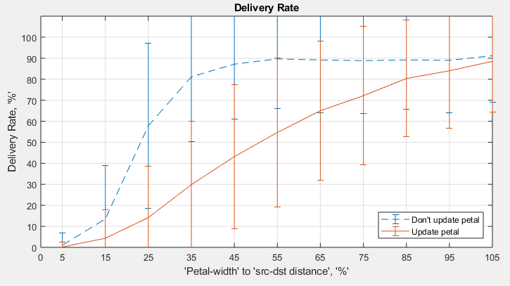
\includegraphics[width=\simResultFigSize \textwidth]{ncsuthesis-0.6/Chapter-5/figs/pe_DR_random.png}
\caption{Delivery rate in random formation}
\label{fig:pe_DR_random}
\end{figure}

\textbf{Packet delivery ratio (PDR):} is defined as the ratio of `count of all packets successfully delivered ($P_r$)' to `count of all the packets transmitted by the sender (P)'. PDR characterizes the robustness and reliability of a routing scheme. The bigger is PDR, the better is the performance of the protocol. 
The packet delivery ratio of flooding algorithm is considered as the upper bound for any routing mechanism since if the destination node is reachable then the probability of packet delivery is high due to the redundant transmissions. This can be observed in \fref{fig:fl_DR_mesh} which shows a plot of PDR vs Hops to Live (HTL) for our implementation of flooding algorithm. It should be noted that for small HTL values (e.g. HTL = 1) the PDR is low because the destination is more than 2 hops apart from the source and the intermediate nodes don't forward the packets. However as HTL approaches the diameter of the network (HTL > 4) PDR approaches 100\% delivery rate. 

\fref{fig:pe_DR_mesh} shows the PDR of petal routing protocol in a mesh formation. We observe that even for petal width of 5\% and 15\%, the delivery ratio is between 70\% to 90\% which is due to the alignment of intermediate nodes in a straight line from source to destination. As expected the PDR approaches 100\% for higher petal width.

\fref{fig:fl_DR_spherical} shows the PDR of flooding in a spherical formation. The distance between the two furthest nodes is $\approx$ 400 m (diameter of the plume) which again causes the PDR to be low for HTL < 4 and gradually increase to 100\% for HTL > 4. \fref{fig:pe_DR_spherical} depicts the PDR for the single and diverged transmission zones in case of petal routing. Unlike mesh formation here we notice that PDR is low for petal width of 15\% and 25\% which is expected because of the routing void created by the plume. It should be noted that the PDR for diverged transmission zone is higher as compared to single transmission zone for petal width of 35\% and 45\%. This observation supports our hypothesis as presented in Section \ref{diverged_trans_zone}.

Finally, \fref{fig:fl_DR_random} shows the PDR of flooding algorithm for a random distribution of UAVs in the flying space. Unlike mesh and spherical formation the PDR doesn't reach 100\% in random distribution rather stays near 90\% for both flooding and petal routing. We can also observe the effect of a thinning petal near the destination for diverged transmission zone in \fref{fig:pe_DR_random} where a single transmission zone achieves a higher PDR as compared to diverged transmission zone for petal width around 35\%.

\section{Average number of hops}

\begin{comment}
\begin{figure}[hbtp]
\centering
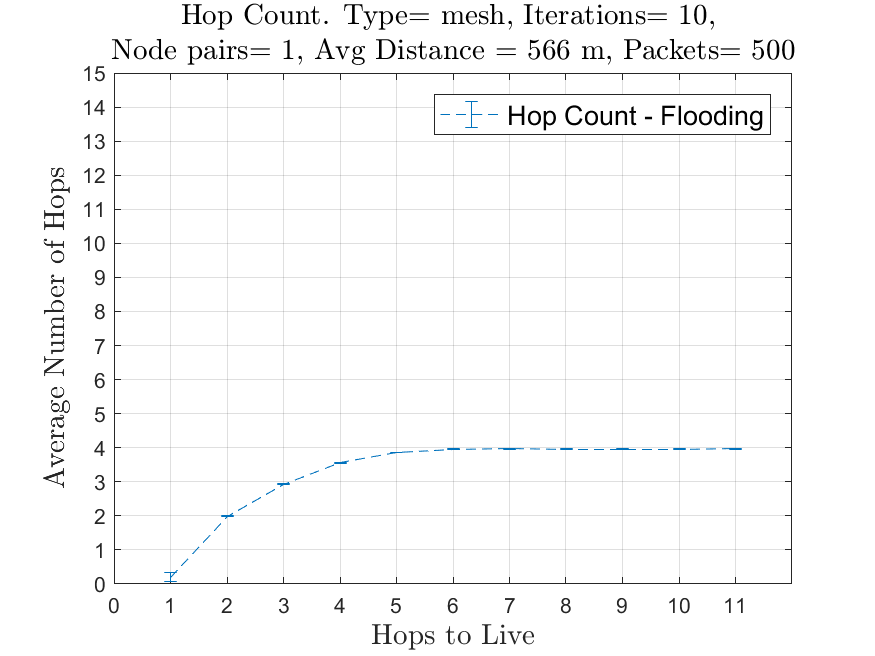
\includegraphics[width=0.8\textwidth]{ncsuthesis-0.6/Chapter-5/figs/fl_hops_mesh.png}
\caption{Number of hops: mesh formation, flooding algorithm}
\label{fig:fl_hops_mesh}
\end{figure}
\end{comment}

\begin{figure}[hbtp]
\centering
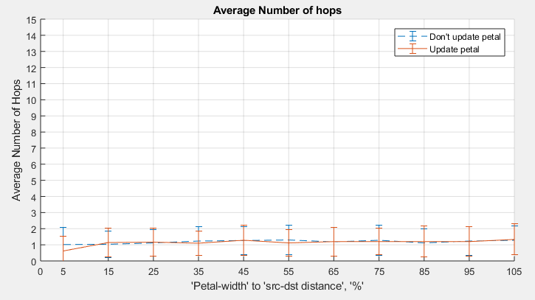
\includegraphics[width=\simResultFigSize \textwidth]{ncsuthesis-0.6/Chapter-5/figs/pe_hops_mesh.png}
\caption{Number of hops in mesh formation for petal routing}
\label{fig:pe_hops_mesh}
\end{figure}

\begin{comment}
\begin{figure}[hbtp]
\centering
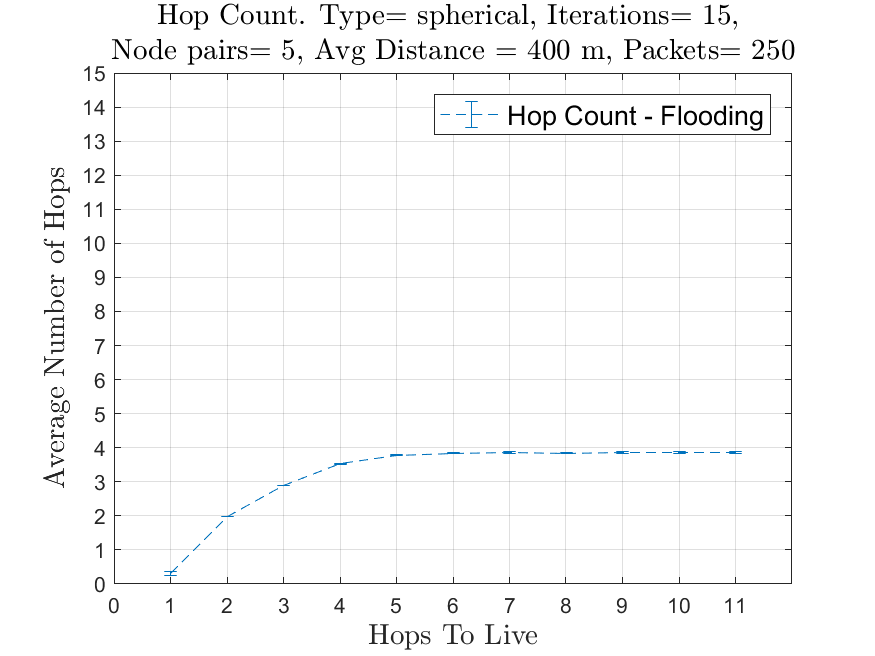
\includegraphics[width=0.8\textwidth]{ncsuthesis-0.6/Chapter-5/figs/fl_hops_spherical.png}
\caption{Number of hops: spherical formation, flooding algorithm}
\label{fig:fl_hops_spherical}
\end{figure}
\end{comment}

\begin{figure}[hbtp]
\centering
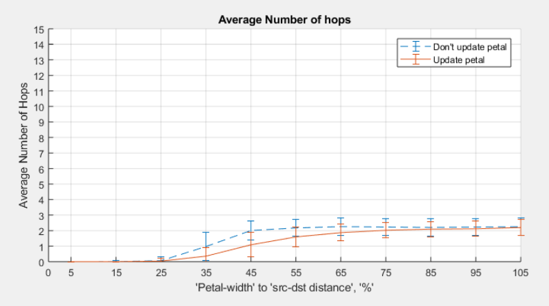
\includegraphics[width=\simResultFigSize \textwidth,height=0.9\textheight,keepaspectratio]{ncsuthesis-0.6/Chapter-5/figs/pe_hops_spherical.png}
\caption{Number of hops in spherical formation for petal routing}
\label{fig:pe_hops_spherical}
\end{figure}

\begin{comment}
\begin{figure}[hbtp]
\centering
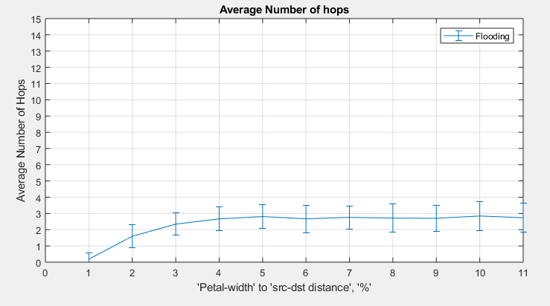
\includegraphics[width=\simResultFigSize\textwidth,height=0.9\textheight,keepaspectratio]{ncsuthesis-0.6/Chapter-5/figs/fl_hop_random.png}
\caption{Number of hops in random formation for flooding algorithm}
\label{fig:fl_hops_random}
\end{figure}
\end{comment}

\begin{figure}[hbtp]
\centering
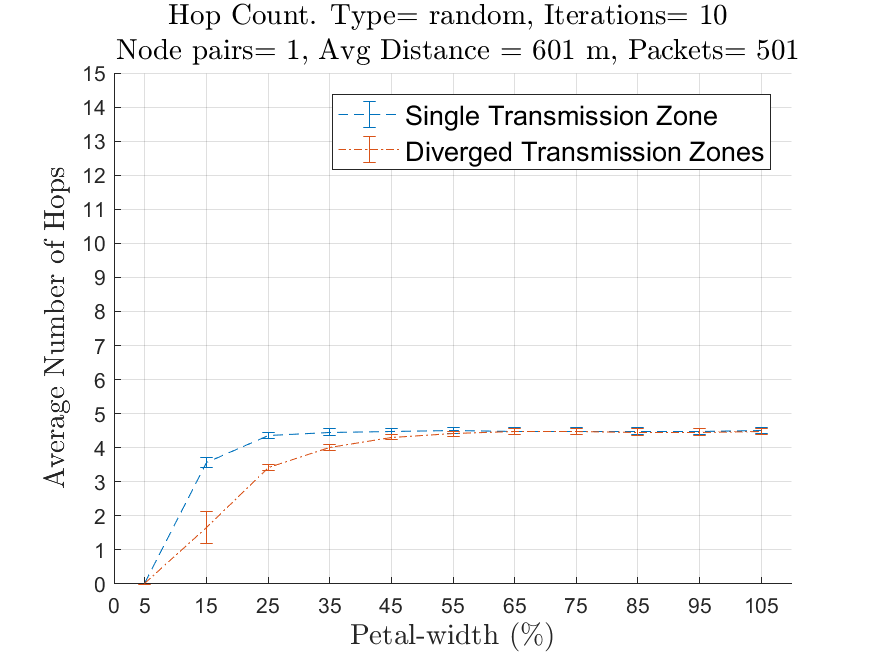
\includegraphics[width=\simResultFigSize\textwidth,height=\textheight,keepaspectratio]{ncsuthesis-0.6/Chapter-5/figs/pe_hops_random.png}
\caption{Number of hops in random distribution for petal routing.}
\label{fig:pe_hops_random}
\end{figure}

\textbf{Average number of hops (H):} is defined as the number of data packets delivered divided by the number of hops performed by all packets. In other words `H' is the number of nodes that transmitted a packet that was successfully delivered to the destination. The number of hops a packet makes before reaching the destination is a representation of the resources consumed in delivering the packet. With antennas having fixed transmitting strength, reducing the number of hops reduces the energy expenditure. Therefore since we have assumed antennas have fixed transmitting strength, a smaller `H' is desired.

\fref{fig:pe_hops_mesh} shows the number of hops made by packets before reaching destination in a mesh formation. Since the nodes are arranged in a straight line even with an inter-drone distance of $\approx 500$ meters the packets reach the destination in about 4 hops. \fref{fig:pe_hops_spherical} plots a similar graph for the spherical distribution. We can see that the number of hops made by packets in  diverged transmission zone is higher for petal width of 35\% and 45\% because the intermediate nodes can route the packets over the spherical void even with thin petal whereas there are not sufficient number of nodes in the other case.

Finally \fref{fig:pe_hops_random} shows the average number of hops made before successful delivery in a random distribution of nodes. Again, we can see that due to thinning of the petal as the packets reach close to the destination the average number of hops is less in random distribution of nodes.

\section{Average end-to-end delay}

\begin{figure}[hbtp]
\centering
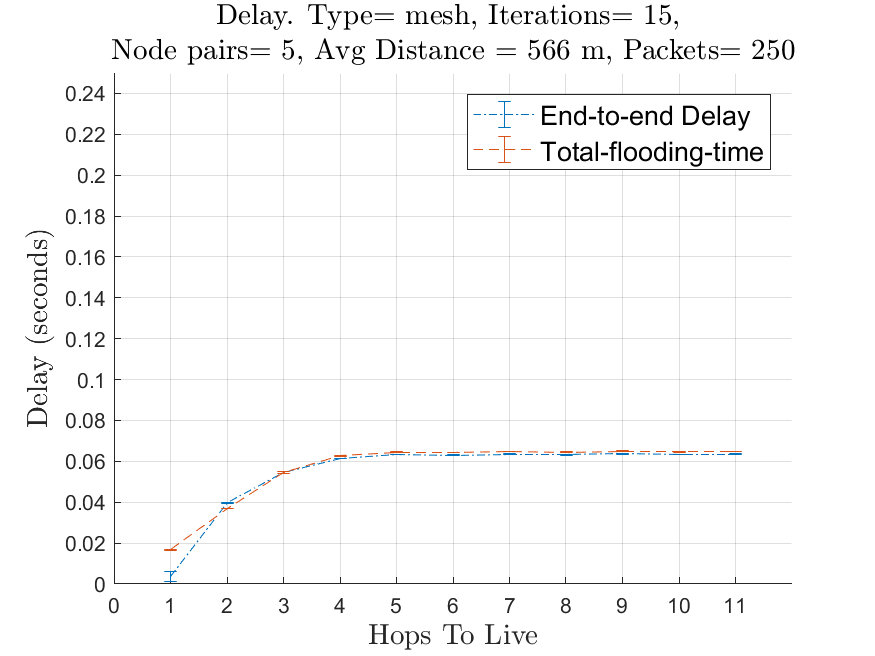
\includegraphics[width=\simResultFigSize\textwidth]{ncsuthesis-0.6/Chapter-5/figs/fl_delay_mesh.png}
\caption{End-to-end delay in mesh formation for flooding. `Total-flooding-time' is the time when all the retransmissions of a packet in the network are over. `End-to-end delay' is the time when the destination node has received the packet.}
\label{fig:fl_delay_mesh}
\end{figure}

\begin{figure}[hbtp]
\centering
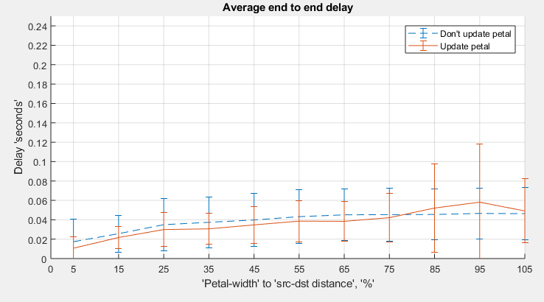
\includegraphics[width=\simResultFigSize\textwidth]{ncsuthesis-0.6/Chapter-5/figs/pe_delay_mesh.png}
\caption{End-to-end delay in mesh formation for petal routing.}
\label{fig:pe_delay_mesh}
\end{figure}

\begin{figure}[hbtp]
\centering
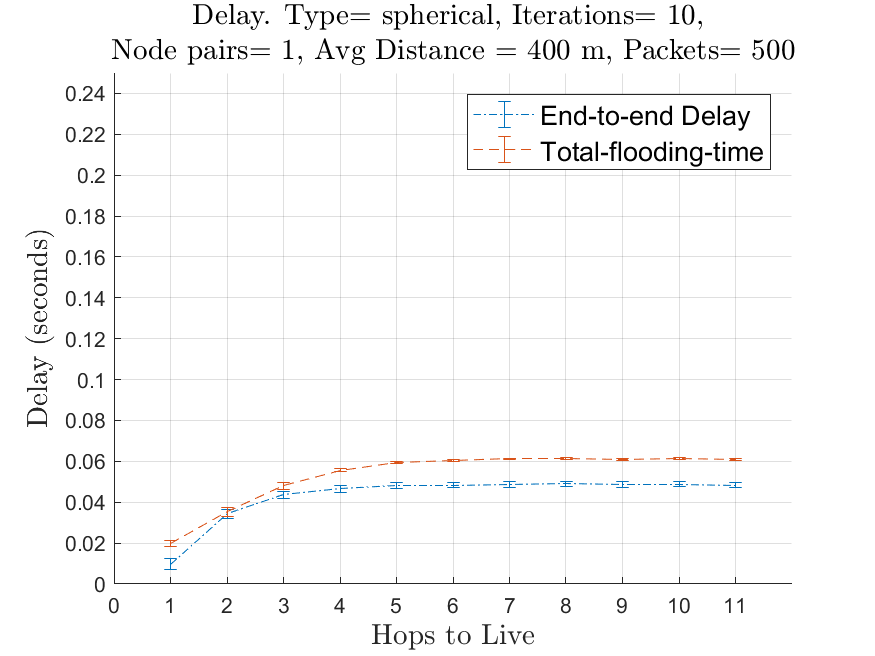
\includegraphics[width=\simResultFigSize\textwidth]{ncsuthesis-0.6/Chapter-5/figs/fl_delay_spherical.png}
\caption{End-to-end delay in spherical formation for flooding. }
\label{fig:fl_delay_spherical}
\end{figure}

\begin{figure}[hbtp]
\centering
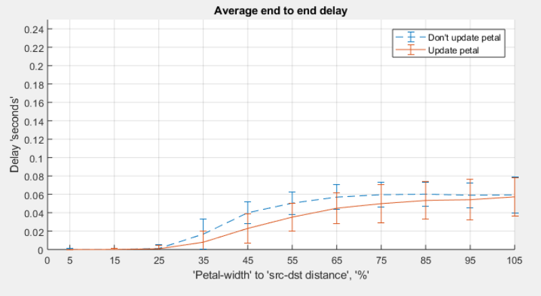
\includegraphics[width=\simResultFigSize\textwidth]{ncsuthesis-0.6/Chapter-5/figs/pe_delay_spherical.png}
\caption{End-to-end delay in spherical formation for petal routing.}
\label{fig:pe_delay_spherical}
\end{figure}

\begin{figure}[hbtp]
\centering
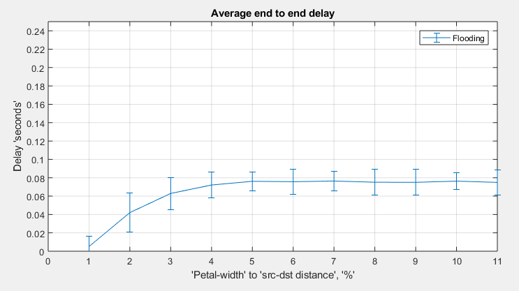
\includegraphics[width=\simResultFigSize\textwidth]{ncsuthesis-0.6/Chapter-5/figs/fl_delay_random.png}
\caption{End-to-end delay in random formation for flooding.}
\label{fig:fl_delay_random}
\end{figure}

\begin{figure}[hbtp]
\centering
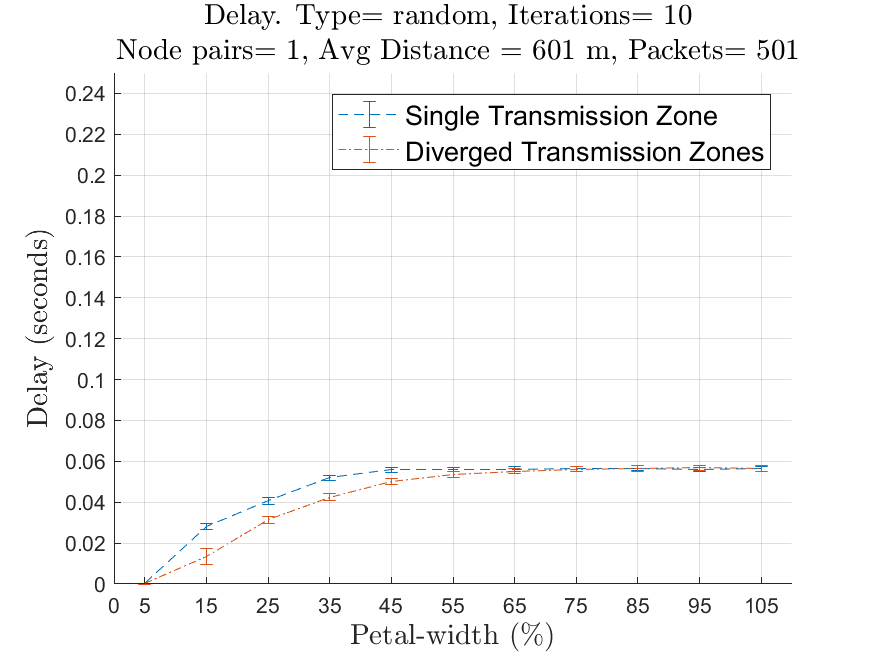
\includegraphics[width=\simResultFigSize\textwidth]{ncsuthesis-0.6/Chapter-5/figs/pe_delay_random.png}
\caption{End-to-end delay in random formation for petal routing.}
\label{fig:pe_delay_random}
\end{figure}

\textbf{Average end-to-end delay (EED):} is defined as the average time for data packets to reach the target destination. Only the data packets successfully received and generated are counted. The smaller is EED, the better is the performance of the protocol. End-to-end delay characterizes the tolerable delay in the network. The EED should be as low as possible to support real-time traffic. This metric is more important in UAV missions like live surveillance or disaster monitoring.

In case of flooding, we have studied the end-to-end delay (i.e. the difference between the time a packet was generated to the time it was received at the destination) and total flooding time (i.e. the time until all transmissions are over and the flooding completes) vs HTL. In other words, Total flooding time represents the time taken when all the re-transmissions for a particular packet in the network are over. For example, if a source and destination node pairs are one-hop neighbors then end-to-end delay shall be low however total-flooding time shall be higher due to the redundant transmissions of the packet in the network. It should be noted that the plots for petal routing depict the equivalent of total-flooding-time in case of petal routing.  

\fref{fig:fl_delay_mesh} represents the delay for flooding algorithm in a 2 dimensional mesh formation. We can see that `End-to-end delay' is equal to 'total-flooding-time' because the number of hops to the destination is equal to the network diameter. \fref{fig:pe_delay_mesh} represents the delay for petal routing in a 2 dimensional mesh formation. The delay for single and diverged transmission zones are approximately equal because of the linear alignment of the nodes. We can notice that the delay is $\approx 0.06$ seconds for flooding and $\approx 0.08$ for petal routing. In case of petal routing the delay accounts for the back-off time (Section \ref{back_off_time}) at each intermediate node.

\fref{fig:fl_delay_spherical} shows the delay in a spherical formation for flooding algorithm whereas \fref{fig:pe_delay_spherical} shows the delay for petal routing. In \fref{fig:pe_delay_spherical} the EED is zero for petal width < 30\% because the denominator --- the number of packets delivered to destination --- is zero. 
Finally \fref{fig:fl_delay_random} and \fref{fig:pe_delay_random} show the delay for random distribution of nodes. 

\section{Average number of transmissions}

\begin{figure}[hbtp]
\centering
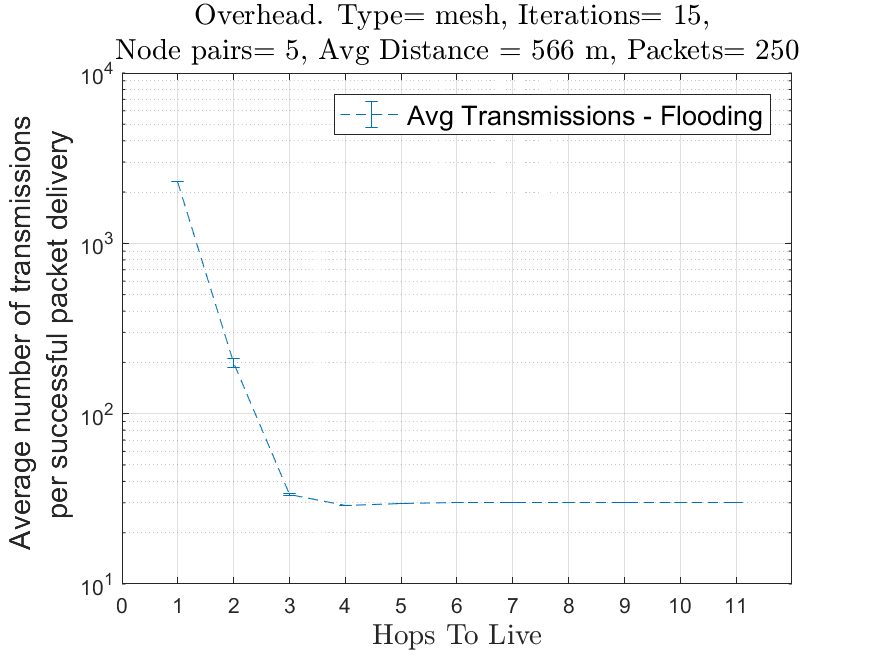
\includegraphics[width=\simResultFigSize\textwidth,height=\textheight,keepaspectratio]{ncsuthesis-0.6/Chapter-5/figs/fl_trans_mesh.png}
\caption{Number of transmissions: mesh formation, flooding algorithm}
\label{fig:fl_trans_mesh}
\end{figure}

\begin{figure}[hbtp]
\centering
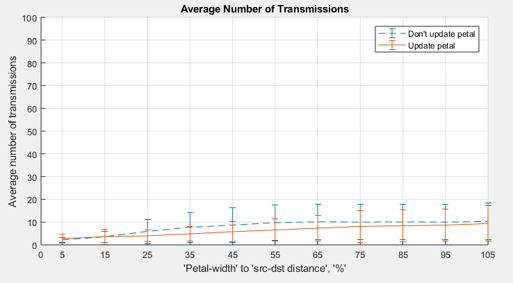
\includegraphics[width=\simResultFigSize\textwidth,height=\textheight,keepaspectratio]{ncsuthesis-0.6/Chapter-5/figs/pe_trans_mesh.png}
\caption{Number of transmissions: mesh formation}
\label{fig:pe_trans_mesh}
\end{figure}

\begin{figure}[hbtp]
\centering
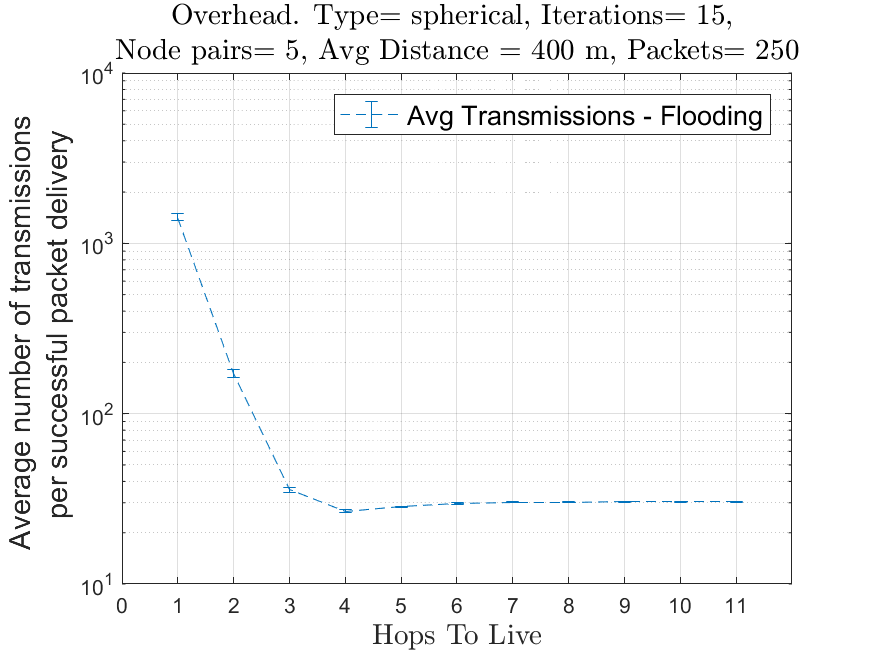
\includegraphics[width=\simResultFigSize\textwidth,height=\textheight,keepaspectratio]{ncsuthesis-0.6/Chapter-5/figs/fl_trans_spherical.png}
\caption{Number of transmissions: spherical formation, flooding algorithm}
\label{fig:fl_trans_spherical}
\end{figure}

\begin{figure}[hbtp]
\centering
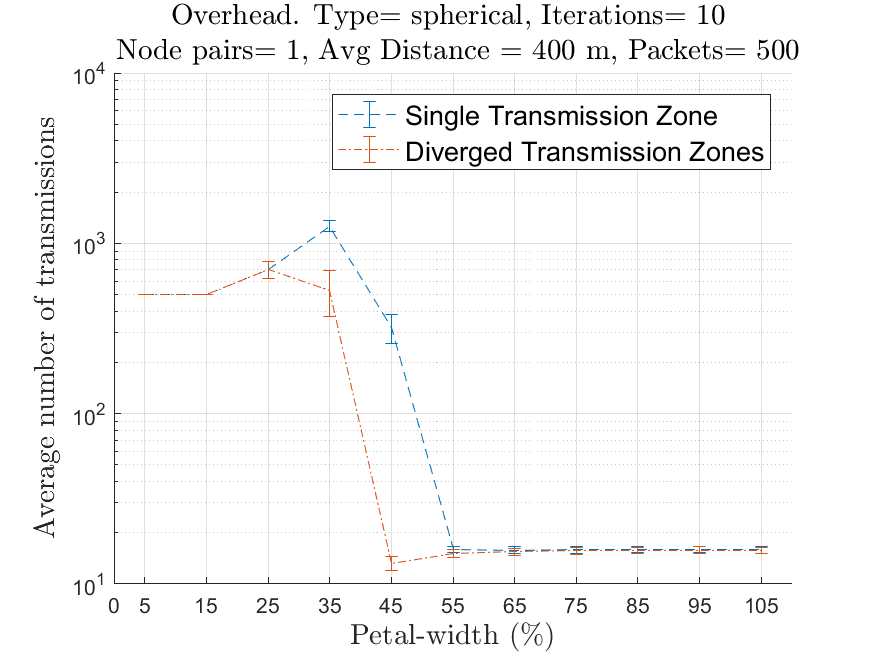
\includegraphics[width=\simResultFigSize\textwidth,height=\textheight,keepaspectratio]{ncsuthesis-0.6/Chapter-5/figs/pe_trans_spherical.png}
\caption{Number of transmissions: spherical formation}
\label{fig:pe_trans_spherical}
\end{figure}

\begin{figure}[hbtp]
\centering
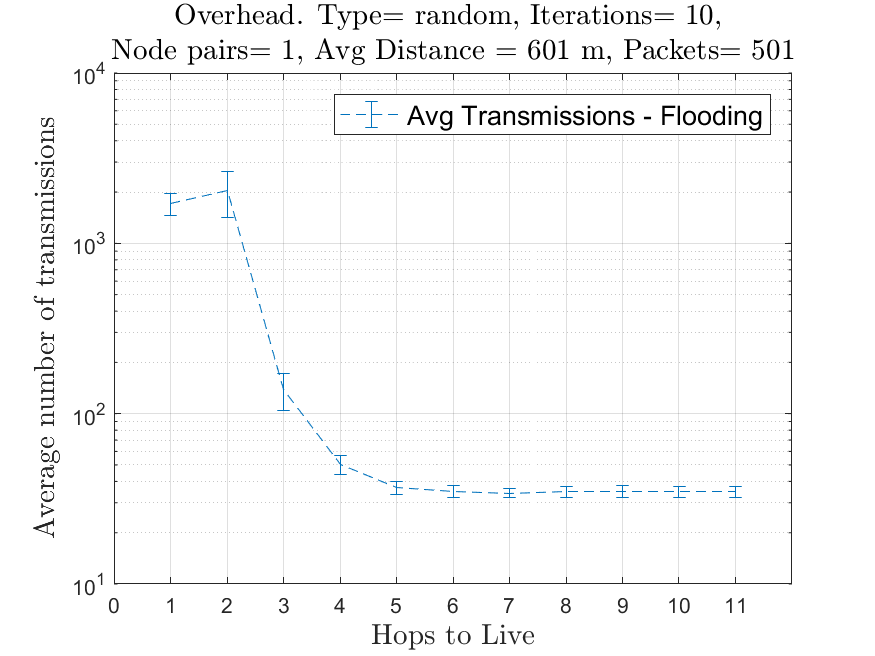
\includegraphics[width=\simResultFigSize\textwidth,height=\textheight,keepaspectratio]{ncsuthesis-0.6/Chapter-5/figs/fl_trans_random.png}
\caption{Number of transmissions: random formation, flooding algorithm}
\label{fig:fl_trans_random}
\end{figure}

\begin{figure}[hbtp]
\centering
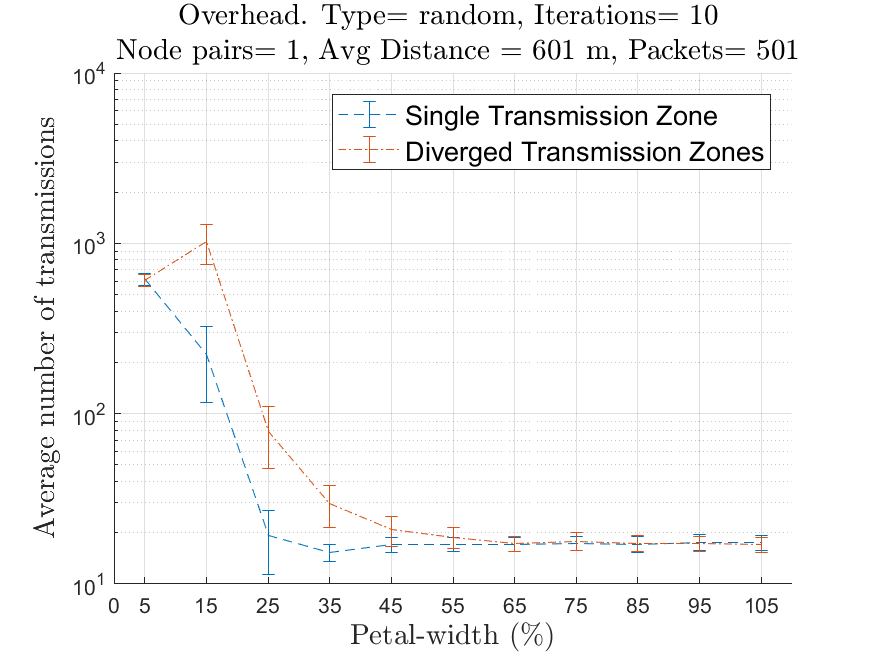
\includegraphics[width=\simResultFigSize\textwidth,height=\textheight,keepaspectratio]{ncsuthesis-0.6/Chapter-5/figs/pe_trans_random.png}
\caption{Number of transmissions: random formation}
\label{fig:pe_trans_random}
\end{figure}

\textbf{Average number of transmissions (NT):} is defined as the total number of transmissions divided by the total number of packets successfully delivered. In an ideal routing protocol `NT' would be equal to `number of hops' $\times$ `number of packets delivered'. In other words number of transmissions is the combined transmissions from all nodes for each successful packet delivery. `NT' directly influences the energy spent in routing a packet also lower number of transmissions leads to lesser collisions in a wireless medium. Hence, a lower value of `NT' is desirable. 

For any packet the upper bound of `NT' is the total number of nodes in the network (because each node transmits the packet at most once). This can be noticed for flooding algorithm in \fref{fig:fl_trans_mesh} where NT is approximately equal to ($ \approx 30$) the total number of nodes ($ = 36$). whereas in our routing algorithm (\fref{fig:pe_trans_mesh}) the number of transmissions drops significantly (about half of flooding) due to the restricted flooding and `back-off and transmit' strategy. It should be noted that if the delivery rate is low the average number of transmissions gets high hence we see the large values for small HTL or thin petal widths.

\section{Effect of network density}

\begin{figure}[hbtp]
\centering
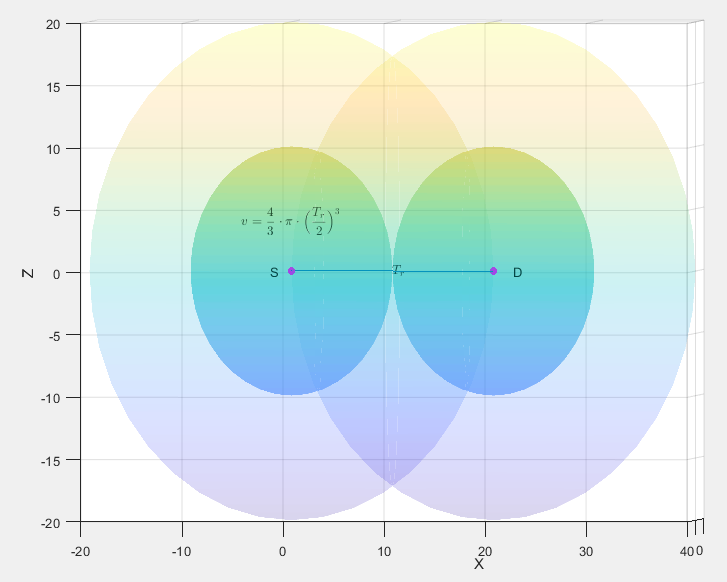
\includegraphics[width=\simResultFigSize\textwidth]{ncsuthesis-0.6/Chapter-5/figs/nodeDensity}
\caption{Compact node alignment for critical network density}
\label{fig:node_density}
\end{figure}

\textbf{Network density:} To achieve a reliable multi-hop communication among the network nodes, the maximum separation between any two nodes should be less than the transmission radius of the transmitting antenna. Therefore --- assuming omnidirectional antennas with transmission radius $T_r$ --- an optimal number of nodes will result in a crystal like packing of space --- the sphere being a node's zone of influence with the node at its center and $\frac{T_r}{2}$ as its radius. This is depicted in \fref{fig:node_density}. A lower number of nodes will result in less reliable communication whereas higher number will result in redundant transmissions and collisions. Hence, we define network density as the ratio of the volume of flying space to the combined volume of the node's sphere of influence. i.e. 

\begin{equation}
    Node Density = \dfrac{L \times W \times H}{ \text{nodeCount} \times \frac{4}{3} \times \pi \times \big(\frac{T_r}{2} \big)^3}
\end{equation}

and we classify the network as sparse, critical and dense as per the following criteria.
\begin{eqnarray} \label{node_density}
\begin{aligned}
& \text{Sparse:} & < 0.8 \\
& \text{Critical:} & \big[0.8, 1.2 \big]  \\
& \text{Dense:} & > 1.2
\end{aligned}
\end{eqnarray}

For example, with scaling factor = 4, Number of Drones = 43, and flying space volume = $ 80 \times 80 \times 40 unit^3  \text{and } T_r = 90 m $,
\begin{eqnarray*}
& \text{we have,} & V = 80 \times 80 \times 40 \times 64 = 16384000 unit^3 \\
& \text{and} & v = 43 \times \dfrac{4 \times 3.14 \times (\frac{90}{2}) ^ 3}{3} \approx 16404930 unit ^ 3 \\
& \Rightarrow \text{Network Density} = & \dfrac{V}{v} \approx 1
\end{eqnarray*}

With 36 drones, the network density is about 1.2, hence the metrics we presented in the previous sections were for critical network density. In this section we shall study the effect of network density on the performance our routing scheme and flooding.

As we observed in Section \ref{pdr}, the PDR for flooding algorithm depends on the HTL and is $>90\%$ for $HTL>4$ whereas PDR depends on petal width in case of petal routing and $>90\%$ for $width>35\%$. 
Therefore, to study the effects of network density we have picked HTL = 10 for flooding and petal width = 35\% for petal routing. 

\fref{fig:nd_DR} shows the variation in delivery ratio vs network density. We can observe that the PDR for flooding is close to that of single transmission zone scheme of petal routing even for sparse network density. This demonstrates the robustness of petal routing i.e. even in sparse networks the reliability of petal routing is as good for flooding for appropriate petal width.

\begin{figure}[hbtp]
\centering
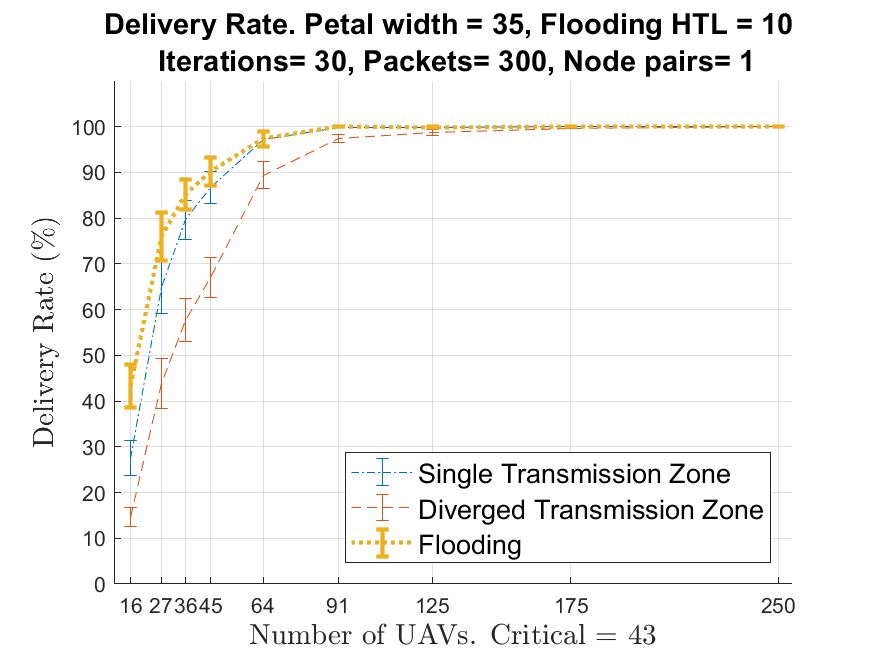
\includegraphics[width=\simResultFigSize\textwidth]{ncsuthesis-0.6/Chapter-5/figs/ND_DR}
\caption{Delivery rate vs network density}
\label{fig:nd_DR}
\end{figure}

\begin{figure}[hbtp]
\centering
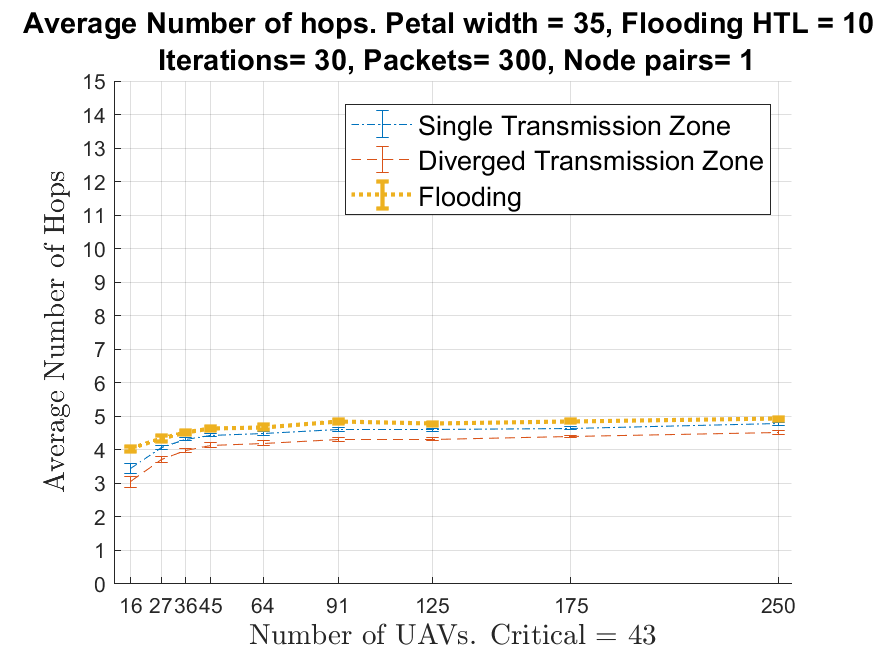
\includegraphics[width=\simResultFigSize\textwidth]{ncsuthesis-0.6/Chapter-5/figs/ND_hops}
\caption{Average number of hops vs network density}
\label{fig:ND_hops}
\end{figure}

\fref{fig:ND_hops} depicts the change in average number of hops as compared to the network density. We can observe that the number of hops doesn't vary much with increase in network density. This is also expected since in both the algorithms the packets propagate in a breadth first manner and hence find the shortest path to the destination. 

\begin{figure}[hbtp]
\centering
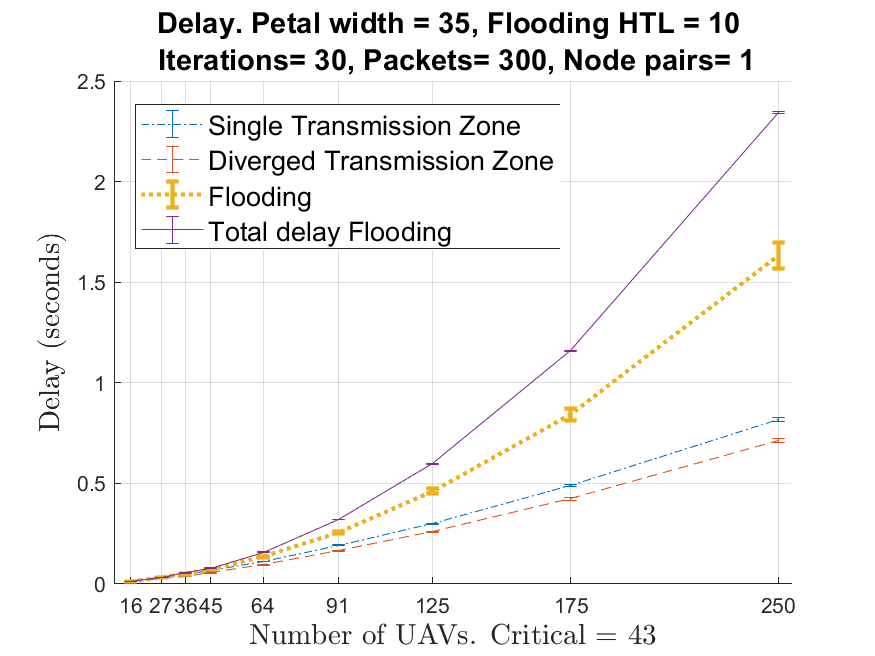
\includegraphics[width=\simResultFigSize\textwidth]{ncsuthesis-0.6/Chapter-5/figs/ND_delay}
\caption{End-to-end delay vs network density}
\label{fig:ND_delay}
\end{figure}

In \fref{fig:ND_delay}, we can observe the change in end-to-end delay with network density. The rate of increase in end-to-end delay for flooding is higher than that of petal routing which is due to the excessive number of retransmissions in the network. Since, our routing algorithm restricts the transmissions to a zone thereby pruning the unnecessary retransmissions.  

\begin{figure}[hbtp]
\centering
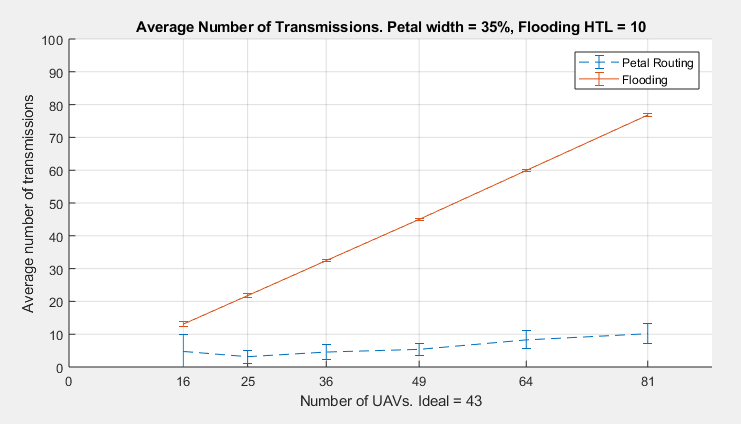
\includegraphics[width=\simResultFigSize\textwidth]{ncsuthesis-0.6/Chapter-5/figs/ND_trans}
\caption{Average number of transmission vs network density}
\label{fig:ND_trans}
\end{figure}

In \fref{fig:ND_trans} we observe that the average number of transmissions increases with increase in network density. However, the increase is more steep for flooding algorithm as compared to petal routing. Specifically, for flooding algorithm, the average number of transmissions is roughly equal to the number of nodes in the network. This is expected since all the nodes which receive a packet transmit at least once in case of flooding; however, in our routing scheme we restrict the retransmissions to a zone and by back-off mechanism as well.

